\documentclass[tikz]{standalone}
\input{common/tikzBase}
\usetikzlibrary{}
\lstset{
    language=C,
    morekeywords=item,
    style=smaller,
    moredelim={**[is][\btHL<2>]{~2~}{~end~}},
}
\newsavebox{\intOverflowExCode}
\begin{document}
\begin{lrbox}{\intOverflowExCode}
\begin{lstlisting}
void vulnerable() {
  int items[100];
  int count;
  bool success =
    try_read_input(&count);
  if (!success) { ... }
  if (count * sizeof() >= sizeof(items)) {
    printf("cannot handle that many\n"); return;
  }
  for (int i = 0; i < count; i += 1) {
    if (!try_read_input(&items[i])) { 
      printf("preature end of input\n"); return;
    }
  }
  process_items(items);
}
\end{lstlisting}
\end{lrbox}

\setSlide{1}
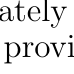
\begin{tikzpicture}
\node[anchor=north east] (code) at (-1,0) {
\usebox{\intOverflowExCode}
};
\node [overlay,draw,very thick,align=left,anchor=north west,font=\fontsize{12}{13}\selectfont] at ([yshift=.5cm,xshift=-6.25cm]code.north east) {
assume return address immediately after items array: \\
Q: what first input number to provide? \\
Q: how to encode return address \\
replacement \texttt{0x12345678}?
};
\end{tikzpicture}
\end{document}
